\documentclass{article}
\usepackage{graphicx} % Required for inserting images
\usepackage[a4paper, total={6in, 8in}, margin=1in]{geometry}
\usepackage{listings}
\usepackage{hyperref}
\usepackage{float}
\usepackage{parskip}
\usepackage{minted}
\usepackage{fontawesome}
\usemintedstyle{vs}
\newcommand{\ts}{\textsuperscript}



\title{Project 2 – INF264}
\author{Felix Anthonisen & Jakob Sverre Alexandersen}
\date{September 21 2024}

\begin{document}

\maketitle
% \newpage
\thispagestyle{empty}

\hfill \break
\hfill \break
\begin{figure}[H]
    \centering
    
\includegraphics[width=0.5\linewidth]{ugle.png}
\end{figure}
\newpage
\maketitle

\section{Summary}

Click me: \href{https://github.com/FelixAnthonisen/INF264-project2}{\faicon{github}} for the full repo

\hrulefill

This project explores the use of machine learning techniques to predict handwritten hexadecimal digits from images. The work is divided into three key parts.

In the first part, we performed hyperparameter tuning and model selection using two classifiers: K-nearest neighbors (KNN) and convolutional neural networks (CNN). The goal was to identify the model that provided the highest prediction accuracy. Our results showed that the CNN outperformed KNN, achieving a test F1-score of 0.954 on unseen data.

In the second part, we applied Principal Component Analysis (PCA) to reduce the dimensionality of the dataset. We aimed to assess how dimensionality reduction impacts both model performance and computational efficiency. By reducing the feature set from 400 to 108 dimensions while retaining 90\% of the variance, we significantly sped up the hyperparameter tuning process—from 2m 19s to  50s—while slightly improving the score on unseen data. The model trained on the full (SMOTEd) dataset achieved a test F1 score of 0.8699, while the reduced dataset model achieved 0.8708.

Finally, in the third part, we were tasked with addressing a corrupted dataset containing out-of-distribution (OOD) images. These OOD images represented clothing, and the objective was to correctly identify as many as possible. To tackle this, we repurposed the CNN model from the first part. By inputting each image from the corrupted dataset into the model and analyzing the activation levels of the most active neuron in the output layer, we could gauge the model’s confidence in its predictions. A high activation indicated a strong probability that the image was correctly labeled, while a low activation suggested a low probability. We used this insight to classify an image as OOD when its activation fell below a predetermined threshold. This approach proved fairly effective, allowing the model to correctly detect 62 out of 85 OOD images. Although increasing the threshold could have detected more OOD images, it would have also raised the number of false positives, which is why we chose not to adjust it further.

Based on our results, we argue that the machine learning approach, particularly using convolutional neural networks (CNNs), is suitable for predicting handwritten hexadecimal digits. The significant accuracy achieved—over 95\% on unseen data—demonstrates that this method effectively captures the patterns inherent in the data.

However, the performance in real-life applications may vary, especially when confronted with corrupted datasets or out-of-distribution images. While our approach to handling OOD images showed some promise, it highlighted the challenges associated with accurately classifying data that deviates from the training set.

Additionally, the suitability of this approach largely depends on the criticality of accuracy in specific applications. If near 100\% accuracy is necessary, this model may not be adequate, and more advanced models or techniques would need to be developed. In summary, while the machine learning approach shows potential for high accuracy, real-world performance will depend on the specific accuracy requirements and the quality and variability of the data to ensure reliability in practical applications.


\subsection{Division of labour}

We both worked in parallel when writing this project. The only times we worked not together was during small optimizing steps and fixing typos.

\section{Data analysis}

We start off by exploring what kind of data we are dealing with, and how the distribution between classes lies:

\begin{figure}[H]
    \centering
    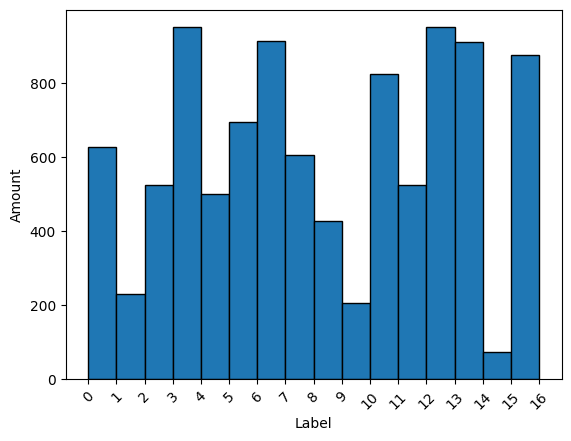
\includegraphics[width=1\linewidth]{distribution.png}
\end{figure}

As you can tell, this dataset is heavily imbalanced, especially for the classes with labels 1, 9, and 14. This can prove to be a challenge as imbalanced datasets can lead to biased models that perform poorly on underrepresented classes. In this case, the model may struggle to accurately identify the classes with fewer examples, potentially resulting in lower accuracy and recall for those specific labels.

\newpage

\begin{figure}[H]
    \centering
    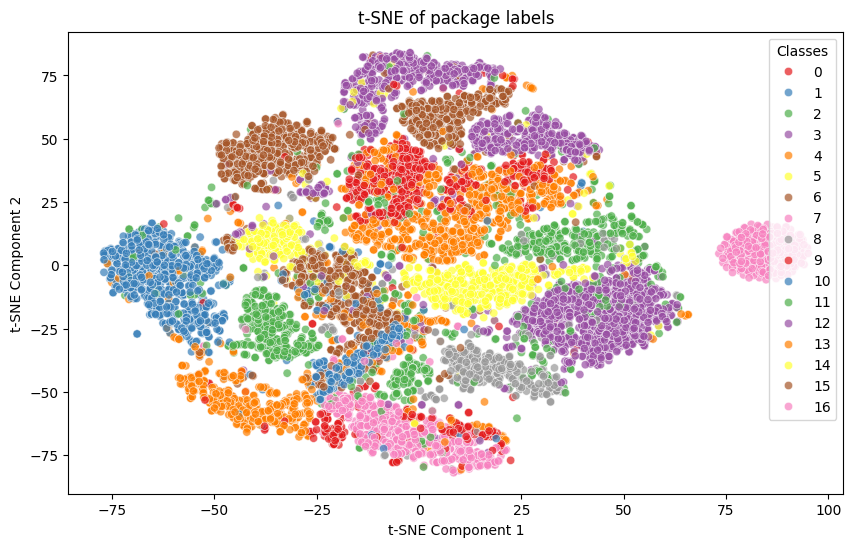
\includegraphics[width=1\linewidth]{tsne.png}
\end{figure}

The clusters group together somewhat nicely. The observant reader may see that the classes 4 and 9 (here, red and orange, respectively) overlap quite a lot. This follows that the digits 4 and 9 share similarities. Oddly enough, we don't see the same patterns with the digits 3 and 8.

\section{Problem 1 – Digit Recognizer}

In this problem, we encounter the task of classifying the types of gifts. We solve this problem with a CNN and a kNN classifier.

The reason we chose a CNN classifier is because they have a good reputation on image classification and was therefore expected to perform well for this task. The kNN classifier was chosen because we saw good clustering on the t-SNE plot, leading us to believe that the kNN model would perform moderately well, although we suspected it would struggle on the aforementioned overlapping classes. It was also chosen because of it's simplicity.

We considered using a Support Vector Machine (SVM) or a Fully Connected Neural Network (MLP), which probably would have performed pretty decently for this purpose. However, we chose not to experiment with those because we had limited time and resources. MLPs also lack the architectural advantage of CNNs for image data, as they treat each pixel independently and don’t capture spatial relationships effectively. For this reason, CNN was expected to outperform MLP.

\subsection{Scaling the dataset}

Before doing anything with the data we chose to scale it. This for a number of reasons:

Gradient Descent converges faster when features are on a similar scale. This can significantly reduce the time it takes to train the model. 

Distance-Based Algorithms: For algorithms that rely on distance metrics (like kNN – our second model), unscaled data can lead to misleading distances. Features with larger ranges will dominate the distance calculation, skewing the results.

Scaling the dataset before using SMOTE (Synthetic Minority Over-sampling Technique) is important because  it uses a KNN model for deciding which images to  interpolate, scaling preserves relationships and improves interpretability.

\textbf{Preserving Relationships:} Scaling helps maintain the relative distances and relationships between data points. Without scaling, the synthetic samples generated by SMOTE might not reflect the actual distribution of the minority class accurately.

\textbf{Interpretability:} Scaling can enhance the interpretability of the model by ensuring that feature importance is evaluated on a consistent scale, allowing for clearer insights into which features are most influential.


\subsection{Balancing the dataset}

Because the dataset is imbalanced, we experiment with the usage of the synthetic oversampling technique SMOTE. This technique generates synthetic samples for the minority class by interpolating between existing samples, helping  to balance the class distribution and improve the model's ability to learn from underrepresented examples. This may lead to better performance in classification tasks, particularly in terms of recall and overall predictive accuracy.

The following image displays some synthetic samples from the expanded dataset.

\begin{figure}[H]
    \centering
    \includegraphics[width=0.75\linewidth]{smote_pics.png}
\end{figure}

As we can see, the generated samples closely resemble the original data, and should therefore be suitable to use for our training.

\subsection{Model selection and tuning}

We employed k-fold cross-validation with k = 5 to reduce overfitting and obtain more reliable performance estimates. The choice of k = 5 represents a balanced compromise between computational cost and estimation reliability - while higher k values (e.g., k = 10) might provide slightly more robust estimates, they also increase computational overhead.

We performed hyperparameter tuning on four different model configurations: kNN and CNN, each tested both with and without SMOTE preprocessing. GridSearchCV was utilized to systematically explore the hyperparameter space for each model configuration. For each model, we  explored hyperparameters listed in subssection 3.4 and 3.5.

Model selection was primarily based on the highest cross-validation score achieved during hyperparameter tuning, as this metric provides a robust estimate of the model's generalization performance. The cross-validation scores helped ensure that our selected model would maintain consistent performance across different subsets of the data, reducing the risk of selecting a model that performed well by chance on a single train-test split.

\newpage

\subsection{kNN hyperparameters}

\begin{table}[ht]
    \centering
    \begin{tabular}{|l|l|l|}
        \hline
        \textbf{Hyperparameter} & \textbf{Description}  & \textbf{Possible values} \\
        \hline
        \texttt{n\_neighbors} & The amount of neighbors & \texttt{[1, 2, 3, 4, 5, 7, 10, 15, 20, 30]} \\
        \hline
        \texttt{weights} & Neighbor voting weight function & \texttt{[uniform, distance]} \\
        \hline
        \texttt{metric} & Distance calculation metric & \texttt{[euclidean, manhattan]} \\
        \hline
    \end{tabular}
    \caption{Possible hyperparameters for the kNN model}
\end{table}

\subsection{CNN hyperparameters}

\begin{table}[ht]
    \centering
    \begin{tabular}{|l|l|l|}
        \hline
        \textbf{Hyperparameter} & \textbf{Description}  & \textbf{Possible values} \\
        \hline
        \texttt{learning\_rate} & Learning rate per epoch & \texttt{[0.001, 0.0005, 0.00025]} \\
        \hline
        \texttt{num\_epochs} & Amount of iterations & \texttt{[10, 20, 30]} \\
        \hline
    \end{tabular}
    \caption{Possible hyperparameters for the CNN model}
\end{table}

\subsection{CNN flow}

\begin{enumerate}
    \item \textbf{Input Layer:}
    \begin{itemize}
        \item The input image is reshaped to be compatible with CNN (a gray-scale image of size $20 \times 20$ is reshaped to \texttt{({batch\_size}, 1, 20, 20)}
    \end{itemize}
    
    \item \textbf{Convolutional Layers (\texttt{conv1} and \texttt{conv2})}
    \begin{itemize}
        \item The first convolutional layer (\texttt{conv1}) applies 16 filters to the input, producing 16 feature maps. These feature maps highlight different aspects of the image (e.g., edges or textures).
        \item The second convolutional layer (\texttt{conv2}) applies 32 filters to the feature maps produced by the first layer, generating more complex features.
    \end{itemize}
    
    \item \textbf{Activation Function (\texttt{ReLu}):}
    \begin{itemize}
        \item The ReLu activation introduces non-linearity after each convolutional layer to allow the model to capture and learn more complex features.
    \end{itemize}

    \item \textbf{Pooling Layers (\texttt{MaxPool2d}):}
    \begin{itemize}
        \item The pooling layer downsamples the feature map, reducing the size of the data while retaining the most important features. In our case it halves the dimensions of the layer.
    \end{itemize}
    
    \item \textbf{Flattening:}
    \begin{itemize}
        \item After the final convolutional and pooling layers, the feature maps are flattened into a single vector to pe passed into the fully connected layers.
    \end{itemize}
    
    \item \textbf{Fully Connected Layers (\texttt{fc1}, \texttt{fc2} and \texttt{fc3}):}
    \begin{itemize}
        \item These layers interpret the abstract features produced by the convolutional layers and generate class scores. The last fully connected layer (\texttt{fc3}) outputs the final class probabilities for classification.
    \end{itemize}
    
    \item \textbf{Dropout:}
    \begin{itemize}
        \item Dropout is applied during training to prevent overfitting by disabling $25\%$ of neurons randomly.
    \end{itemize}
    
    \item \textbf{Output Layer (\texttt{fc3}):}
    \begin{itemize}
        \item This layer gives the final classification score for each class.
    \end{itemize}
\end{enumerate}

\newpage

\subsection{Classifier results}

We used \texttt{f1\_score} to score our classifiers. The reason for this is because the dataset is unbalanced, meaning that one class is significantly more frequent than the other. In such cases, accuracy can be misleading as it may favor the majority class. The F1 score, which is the harmonic mean of precision and recall, is better suited for evaluating models on unbalanced data. It provides a balance between the classifier's ability to correctly identify the positive instances (precision) and its ability to capture as many positive instances as possible (recall). This makes the F1 score a more reliable metric for assessing the performance of our classifiers on this unbalanced dataset.

\begin{table}[ht]
    \centering
    \begin{tabular}{|l|l|}
        \hline
        \textbf{Classifier} & \textbf{Validation F1 score} \\
        \hline
        \texttt{CNN} & 0.9491 \\
        \hline
        \texttt{kNN} & 0.8677 \\
        \hline
        \texttt{CNN with SMOTE} & 0.9497 \\
        \hline
        \texttt{kNN with SMOTE} & 0.8355 \\
        \hline
    \end{tabular}
    \caption{Results for all classifiers}
\end{table}

We observe that the CNN (Convolutional Neural Network) model achieved an F1 score of 0.9491, while the k-Nearest Neighbors (kNN) model scored 0.8677. After applying SMOTE, the CNN’s F1 score slightly improved to 0.9497, suggesting that the class balancing technique had a positive, albeit minimal, effect. In contrast, the kNN model’s F1 score decreased to 0.8355 with SMOTE, indicating that it may not benefit as much from oversampling in this scenario. Overall, the CNN model performs better in both cases, showing its robustness to the original and balanced datasets. 
\begin{table}[ht]
    \centering
    \begin{tabular}{|l|l|}
        \hline
        \textbf{} & \textbf{Value} \\
        \hline
        \texttt{Model name} & CNN with SMOTE\\
        \hline
        \texttt{Learning rate} & 0.001 \\
        \hline
        \texttt{Num epochs} & 30 \\
        \hline
        \texttt{Test F1 score} & 0.954 \\  
        \hline
    \end{tabular}
    \caption{Results for the final model}
\end{table}

The reason why CNN performed better is likely because CNNs are generally better suited for image classification tasks due to their ability to automatically learn spatial hierarchies from raw pixel data. They can capture local patterns, such as edges and textures, and then combine these features at deeper layers to recognize more complex structures within the image. This hierarchical feature extraction process makes CNNs particularly effective for handling image data, where relationships between pixels are crucial for identifying objects or scenes. Additionally, CNNs are robust to variations in scale, position, and orientation within images, further enhancing their suitability for tasks like object detection and image recognition.

In contrast, k-Nearest Neighbors (kNN) is a non-parametric algorithm that does not inherently account for spatial relationships in data. It relies on measuring distances between instances, making it more sensitive to noise and less effective when complex feature interactions are necessary for accurate classification. This limitation is especially pronounced in image data, where high-dimensional pixel features require more sophisticated processing to discern meaningful patterns. Consequently, CNNs outperform kNN in many image-related tasks, where spatial feature extraction is key to success.

In a production environment, we expect the model to perform pretty well, with comparable results to what we got on the test data. This is because the test data was unseen all the way up until evaluating the performance of the classifier, therefore it roughly simulates a production environment. 

\section{Problem 2 – Avoiding the curse of dimensionality}

We create a pipeline to run grid search with PCA. The reason why one would choose to use Principal Component Analysis is to reduce dimensionality in the dataset. By eliminating less important dimensions, PCA can help reduce the noise in the data. Potentially improving both model performance and computational efficiency.

We did not use PCA for the CNN because it is unsuitable, therefore we only applied it to our kNN model.

The grid search is as follows:

\begin{table}[ht]
    \centering
    \begin{tabular}{|l|l|l|}
        \hline
        \textbf{Hyperparameter} & \textbf{Description}  & \textbf{Possible values} \\
        \hline
        \texttt{n\_neighbors} & The amount of neighbors & \texttt{[1, 2, 3, 4, 5, 7, 10, 15, 20, 30]} \\
        \hline
        \texttt{weights} & Neighbor voting weight function & \texttt{[uniform, distance]} \\

        \hline
        \texttt{metric} & Distance calculation metric & \texttt{[euclidean, manhattan]} \\
        \hline
        
        \texttt{n\_components} & Amount of variance we keep & \texttt{[0.9]} \\
        \hline
    \end{tabular}
\end{table}

This gave us the following results on the kNN:

\begin{table}[ht]
    \centering
    \begin{tabular}{|l|l|l|}
        \hline
        \texttt{Model name} & \textbf{kNN PCA} & \textbf{kNN} \\
        \hline
        \texttt{n\_neighbors} & 4 & 4\\
        \hline
        \texttt{weights} & \texttt{distance} & \texttt{distance} \\
        \hline
        \texttt{metric} & \texttt{Euclidian} & \texttt{Euclidian} \\  
        \hline
        \texttt{Test F1 score} & 0.9743 & 0.8675 \\  
        \hline
    \end{tabular}
    \caption{Results for the kNN models – with and without PCA}
\end{table}

Using PCA, we reduced the number of features from 400 to 108. This number was selected to retain 90\% of the variance in the dataset, ensuring that most of the important information was preserved. Another approach could have been to tune the hyperparameter for the optimal number of components, kkk, but due to time constraints in this task, we opted not to pursue that.

PCA proved to be highly efficient, reducing the time for hyperparameter tuning and model selection from 2 minutes 19 seconds to 50 seconds, significantly accelerating the process. This speedup did not compromise model performance. In fact, the best PCA-based kNN model outperformed the best non-PCA model, with a 0.006 score improvement.


\newpage

\section{Problem 3 – Detecting Out-of-Distribution Images}

In problem 3, we were tasked with detecting out-of-distribution (OOD) images in a corrupted dataset. The dataset was similar to those used in previous tasks, containing images of handwritten hexadecimal digits, but also included OOD images featuring items of clothing. The goal was to build a model capable of accurately distinguishing between in-distribution (hexadecimal digits) and OOD (clothing) images.

Our approach to solving this problem involved repurposing the CNN classifier from task 1. To explain how this works, consider an individual image. When this image is passed through the CNN, the model generates activations for each neuron in the output layer, where each neuron corresponds to a particular label. The higher the activation of a neuron, the more confident the model is that the image belongs to the corresponding label. If one neuron shows a strong activation while the others are low, it indicates high confidence that the image is in distribution and fits a known label. Conversely, if all neurons show low activations and no particular label stands out, this could suggest the model is unsure, \href{https://www.youtube.com/watch?v=FU7vA8rVkLA}{perchancely} indicating that the image is OOD. This is the foundation of our way of making predictions. 

To formalize our approach: We pass each image through the CNN and examine the activations in the output layer. If the maximum activation is below a predefined threshold, we classify the image as OOD. Otherwise, we classify it as in-distribution. This method relies on the intuition that low confidence across all output neurons suggests the image might not belong to any of the known classes, indicating it's OOD.

We set the threshold to 9, and this approach yielded reasonably good results. Out of the 94 images labeled as OOD, 62 were true positives (correctly identified as OOD) and 32 were false positives (incorrectly labeled as OOD), giving us an accuracy of 65.96\%. Below are the labeled images.

\begin{figure}[H]
    \centering
    \includegraphics[width=0.75\linewidth]{ood_images.png}
\end{figure}
Many of the false positives were understandable upon closer inspection. These included odd or malformed digits, as well as examples of Greek letters, which were likely unfamiliar to the model. Given their unusual or ambiguous appearance, it's clear why they were flagged as OOD.
\newpage

\section{On overfitting}

Not only is cross-validation a tool we can use to assess different model hyperparameters, but it can also prevent overfitting. Here is how: 

\begin{itemize}
    \item \textbf{Evaluates Model on Multiple Data Subsets: }In $k$-fold cross-validation, the dataset is divided into $k$ folds. The model is trained on $k-1$ folds and tested on the remaining fold. This process is repeated $k$ times, each time with a different fold as the test set. By averaging the results across all folds, you get a more reliable measure of the model’s generalization ability.

    \item \textbf{Reduces Dependence on Specific Training Data:} By training on different portions of the data, cross-validation helps ensure the model doesn't become too dependent on any one subset. This reduces the likelihood that the model will overfit the training data, as it has to perform well across multiple test sets.

    \item \textbf{Provides a More Robust Performance Estimate:} Since cross-validation provides an averaged performance metric, it reflects the model's capability to generalize to new, unseen data. A high variation in scores across folds can indicate a model prone to overfitting, prompting us to adjust the model or hyperparameters accordingly.

\end{itemize}

In summary, cross-validation is an effective way to mitigate overfitting by ensuring that a model is evaluated on multiple data subsets, which leads to a more accurate estimate of its true performance on new, unseen data.

We also incorporate dropout in our CNN. It is a regularization technique that helps prevent overfitting by randomly "dropping out" a proportion of neurons during each training iteration. 

On our CNN architecture, we set the dropout rate to 25\%. This means that 25\% of the neurons get set to zero. In other words, they are temorarily removed from the network for that iteration, along with their connections. However, during testing, dropout is not applied, and our network uses all neurons.

\section{Further improvement}

If we had more time and were allowed to run the production code on CUDA-accelerated machines, we could have increased the amount of hyperparameters in our models. This would also mean that we could increase CNN architecture complexity and try out larger models. If we had done this again, we would have liked to experiment with a \href{https://arxiv.org/pdf/1506.02640}{YOLO} model, R-CNN, Fast R-CNN or maybe even a Faster R-CNN model.

We could also have implemented a different OOD strategy, rather than extracting information from the final fully connected layer of our CNN. Such a strategy could involve selecting a couple images we know for a fact are corrupted and training the model on those in a recursive manner. This would enable us to detect more corrupt images and again select those for further training, all the way until all 85 images have been detected.

$\theta_{n+1} = \theta_{n} - \eta \cdot \nabla \L(D)$

\end{document}